\chapter{Evaluation}

Evaluating whether a project is successful or not is not an easy task \citep{lit:definining_success}. \cite{lit:definining_success} found that the definition of success can vary from a type of stakeholder to another. The definition of success is based on three important indicators: cost, time, and scope (which includes functionality and software quality) \citep{lit:definining_success}. Some stakeholders value the attainment of scope in the desired time, while others consider delivering on time the most important. Overall, \cite{lit:definining_success} found in a survey they conducted that all stakeholders value scope the most.

This chapter will present a critical evaluation of the project. First of all, we will try to check how well was the \textit{scope} met. After that, we will compare the project with existing tools, and finally we will do a practical evaluation of the library, by using exercises from existing sources.

\section{Attainment of \textit{scope}}
According to \cite{lit:definining_success}, scope is generally understood as both functionality and software quality.

\subsection{Functionality}

The required functionality of the application was previously defined in the Requirements chapter. The functionality was split in two parts: the web application and the grading library.

When looking at the functionality required for the web application, we believe that all of the presented requirements have been fully met. Most of these requirements can be manually checked and most these requirements (all with the exception of R1 and R11) are fully tested in the integration test suite. The tests are located under \texttt{spec/features/**\_spec.rb} in the web application source code folder.


However, when looking at the requirements for the grading library, it is much harder to assess the degree to which these were met. Most of the requirements are impossible to measure, especially considering that some of them included a research phase. For instance, evaluating requirements such as ''The library should implement a grading algorithm for assessing SQL assignments'' is realistically impossible. While the library implements such an algorithm, it is very difficult to assess its implementation. Evaluating the library by looking at the functionality implemented is not highly relevant. A more relevant evaluation process of the library is an empirical one, which will be presented later in this chapter.

\subsection{Software quality}

Evaluating software quality is not an easy task as there is no single universally accepted way of measuring quality. Different people define software quality differently: some argue that code coverage is an indication of quality, while others believe that other metrics, such as performing efficiently, how easy can one modify the code, intelligibility of code, etc., are more relevant \citep{msft_testing, Boehm:1976:QES:800253.807736}.

It is our belief that overall the resulting software is of good quality. However, performing a non-empirical evaluation of software quality is not possible. To ensure software quality, we can list some of the considerations the project took:
\begin{itemize}
    \item Ensure that all code is fully tested and that code coverage is 100\%
    \item Ensure that all code adheres to the standards provided by Rubocop to ensure a legible and easy to understand code.
    \item Ensure that security is implemented correctly either by strong encryption or by secure execution of user input.
\end{itemize}

One area where the software quality is not as good as we would have wanted is performance in the grading algorithm, more specifically the canonicalization process. During the transformation step, some queries are executed multiple times (e.g. getting the columns for a table is used by multiple canonicalizations steps). While grading is still very fast, these processes could be further improved to avoid unnecessary database queries.

\section{Comparing the application with existing tools}

When comparing the functionality of the application built with existing tools for automating SQL assessment, the most suitable comparison would be one with XData. While a comparison can also be done with commercial tools or tutor-style applications, the comparison with XData is more relevant as both XData and our tool provide a different, and arguably better, grading algorithm than these tools.

\subsection{Comparison with XData}

The most important comparison with XData can be done on the basis of two criteria: the canonicalization process and the grading algorithm. One important aspect to keep in mind is that while XData also supports sub-queries to a certain degree, our application does not have any form of support for sub-queries.

The canonicalization process is very similar in both apps. The improvements done in our project are fairly limited with only two canonicalizations added. Even with these two added transformations, the reality is that limitations described in section \ref{ch:lit:sec:can:subsec:limit} are still present. In addition, these two transformations do not make any progress on solving the existing issues.

On the other hand, the implemented grading algorithm builds on top of the work done by XData. The newly implemented Boolean component comparison is a new addition that will ensure even more accurate grading. Moreover, the algorithm is able to partially grade two components that do not perfectly match. This will ensure that small mistakes such as using the wrong type of join will not deduct full points.

XData also provides some important additional features that are not included in our application or the scope of the project:
\begin{itemize}
    \item Support for multiple RDBMS: XData has support for Oracle DB, Microsoft SQL, Postgres (it does support MySQL, which is used in our project). By allowing support for multiple RDBMS, XData has the potential of being deployed in more university courses.
    \item XData implements a data generation algorithm that removes the need of seeding dummy data from the teacher. XData automatically creates a set of data based on the teacher's correct query. This feature should prevent situations where two queries return the same result even if they are different. According to \cite{lit:xdata_d}, this data generation has been shown to outperform fixed data-sets.
\end{itemize}

\subsection{Comparison with other tools}
The most important comparison with the other tools can be made based on the user experience. While their grading algorithm might be inferior, the commercial tools provide a much better user experience with a much better design. The UX and UI area of the project did not receive too much attention, due to time constraints and due to the reduced importance compared to the grading algorithm.

For instance, HackerRank provides a much easier web interface to use: challenges are formed of multiple categories, each challenge has a discussion forum, one can easily see its past submissions, etc.

\section{Testing the application against exercises from existing sources}
The most important type of evaluation, in our opinion, is represented by a type of evaluation that tries to understand how practical the application would be in reality. Other tools developed for academia have been tested in actual courses. However, for this smaller project, this has not been possible; therefore, the application has been tested against different assignments from various sources. We looked at exercises from the following two sources.

\begin{itemize}
    \item Exercises from \textit{Database System Concepts, 5th edition} written by Abraham Silberschatz, Henry F. Korth, S. Sudarshan.
    \item Exercises from the HackerRank \texttt{SQL} course.
\end{itemize}

The goal of this evaluation is to understand if the application will be able to handle actual usage if it were to be deployed in production. The evaluation will focus exclusively on the accuracy of the grading algorithm. To assess the accuracy of the algorithm built, an evaluation of its ability to extract comparable components has been performed. We can define  a comparable component as one that was either canonicalized or cannot be rewritten in any other way. This aspect is the the most important one of the application as it directly influences the final grade.

\subsection{Exercises from HackerRank}

As mentioned in \ref{ch:lit:sec:tutor:comercial}, HackerRank provides multiple \texttt{SQL} exercises that can help a student practice their \mintinline{mysql}{SELECT} SQL abilities.

HackerRank separates their SQL course in 5 parts: Basic Select, Basic Join, Advance Select, Advance Join and Aggregate.

For the evaluation, we manually found solutions for the exercises from HackerRank. In addition, we manually wrote the schema creation SQL for each assignment. The solutions and queries were extracted to a \texttt{spec/fixtures/transformer\_hacker\_rank\_integration\_tests.yml} (included in the appendix) file that automatically generates RSpec tests as described in section \ref{ch:impl:sec:testing:subsec:integ_library}. For the queries which are not supported, a \texttt{support: false} is added in their hash.

\subsubsection{Results of evaluation}
The results based on the challenge category are as following:
\begin{enumerate}
    \item \textbf{Basic Select}: Out of 25 queries, 21 have been successfully transformed. The remaining 4 solutions are not transformable due to issues in sql-parser:
    \begin{itemize}
        \item 1 query uses \mintinline{mysql}{COUNT(DISTINCT column)} which is not currently supported
        \item 2 queries use \mintinline{mysql}{length(string)} which is not currently supported. Sql-parser does not support any string functions.
        \item 1 query uses \mintinline{mysql}{substr(string, integer)} which is not currently supported
    \end{itemize}
    \item \textbf{Basic Join}: Out of 10 queries, 7 have been successfully transformed. The remaining 3 queries cannot be transformed for two reasons:
    \begin{itemize}
        \item 1 query uses \mintinline{mysql}{CASE} which is not currently supported by sql-parser
        \item 2 queries use sub-queries
    \end{itemize}
    \item \textbf{Advance select}: Out of 5 queries, only one is supported. The remaining ones encountered the following issues:
    \begin{itemize}
        \item 2 queries use \mintinline{mysql}{CASE} which is not currently supported by sql-parser
        \item 1 query uses \mintinline{mysql}{concat} which is not currently supported by sql-parser
        \item 1 query uses sub-queries
    \end{itemize}
    \item \textbf{Advance join}: Out of 5 queries, only one is currently supported.
    \begin{itemize}
        \item 1 query uses a \mintinline{mysql}{UNION} which is not currently supported by either sql-parser or our algorithm, due to the limitation of using sub-queries
        \item 3 queries use sub-queries
    \end{itemize}
    \item \textbf{Aggregate}: Out of 23 queries, 16 have been fully transformed. The remaining 7 queries cannot be transformed for two reasons:
    \begin{itemize}
        \item 6 queries use the \mintinline{mysql}{ROUND} function, which is not currently supported by sql-parser. Sql-parser does not support any math functions.
        \item 1 query use sub-queries
    \end{itemize}
\end{enumerate}

\begin{figure}
\centering
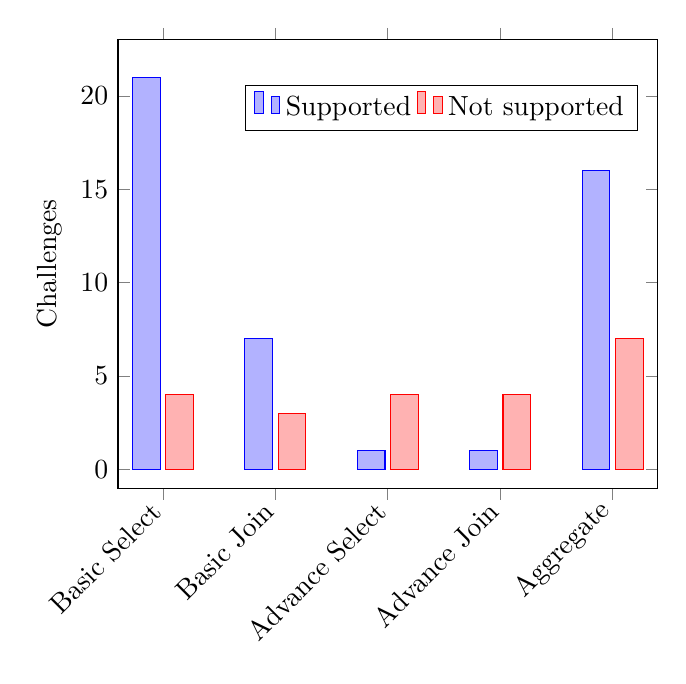
\begin{tikzpicture}
\begin{axis}[
    symbolic x coords={Basic Select, Basic Join, Advance Select, Advance Join, Aggregate},
    ylabel=Challenges,
    ybar,
    x tick label style={rotate=45,anchor=east},
	legend style={at={(0.6, 0.9)},
		anchor=north,legend columns=-1},
    xtick=data]
\addplot coordinates {
    (Basic Select, 21)
    (Basic Join, 7)
    (Advance Select, 1)
    (Advance Join, 1)
    (Aggregate, 16)
};
\addplot coordinates {
    (Basic Select, 4)
    (Basic Join, 3) 
    (Advance Select, 4)
    (Advance Join, 4)
    (Aggregate, 7)
};
\legend{Supported, Not supported}
\end{axis}
\end{tikzpicture}
\caption{Evaluation results with HackerRank exercises}
\label{fig:my_label}
\end{figure}

Overall, out of 68 challenges from HackerRank, the algorithm was able to fully transform 46 of them - a success rate of 67\%. 

The most important issue that showed up during the evaluation process is how limited sql-parser is. We discovered many issues such as not being able to handle column names (if unqouted) that contain SQL commands in them (e.g. COUNTRYCODE would trigger an error as it includes COUNT). In addition, we noticed that sql-parser does not currently support the full SQL language (e.g. methods such as \mintinline{mysql}{LENGTH} were not included, or math rounding functions were not included). While some bugs have been fixed, there are still some bugs that prevent the parsing of queries. The full limitation of sql-parser will be presented in the conclusion chapter, under the limitation section.

Another issue that showed up was the use of sub-queries in complicated queries. We knew before that more advance queries had to use sub-queries to solve the challenge, so this was expected.

\subsection{Exercises from \textit{Database System Concepts, 5th edition}}

\textbf{Database System Concepts} is a textbook for learning about databases. The book has two chapters on SQL that contain 14 exercises with \mintinline{mysql}{SELECT} statements whose solutions are, in our opinion, fairly basic (no complicated SQL functions, or complicated JOIN conditions, etc.). Out of these 14 exercises, more than half (9) contains sub-queries in their solutions. That means that these 9 are currently not supported by our tool. The rest of 5 queries can be transformed to comparable components.

In addition to the \mintinline{mysql}{SELECT} statements, the two chapters about SQL also include \mintinline{mysql}{SELECT} and \mintinline{mysql}{UPDATE} statements. Another interesting observation from looking at exercises from the book is that relational algebra is used throughout the book to teach students database concepts. Furthermore, the book also contains multiple choice questions that are not in the scope of the current project.

\section{Limitations of the evaluation}
\subsection{Resulting grade accuracy}
Throughout the process of evaluation, we only looked at how well the algorithm can extract comparable components. However, we ignored the resulting grade as it is currently impossible for us to properly evaluate if a grade is good or not. To evaluate this, a teacher (or a TA) should compare the algorithm's grades to what grade they would give.

\subsection{Queries tested}
The evaluation process only looked at the ability of the algorithm to extract components from correct or almost correct queries. However, when testing with students, it might be the case that some of them come with solutions totally different that the correct one. It is very hard for us to accurately test this scenario, as the way of solving a problem might be totally different for someone.

\subsection{HackerRrank exercises}
Although HackerRank has over 60 exercises, most of them are very similar. This could affect the evaluation as there were only a few types of errors reported. A more diverse exercise sample would probably result in either more diverse errors, or perhaps in more supported queries.

\section{Conclusion of the evaluation}
After the evaluation process, and especially the evaluation using HackerRank exercises, the following conclusions about the project can be made:
\begin{enumerate}
    \item The parser used (sql-parser) is fairly limited and during the evaluation it represented a major error source. Some bugs found during the evaluation process were fixed, but some are still present.
    \item If the algorithm can successfully parse the queries, it can provide comparable components that can be used to provide an accurate grading.
    \item The partial algorithm is a improved version over XData by providing even more detailed partial grading.
\end{enumerate}

With all these in mind, our belief is that the application in its current form is not yet fully complete. More work has to be done to improve some features, especially the parser and adding support for sub-queries. We think that the approach taken by XData and our project is the correct one to ensure accurate partial grading.